% $Id: solution.tex 1784 2012-04-27 23:29:31Z nicolas.cardozo $
% !TEX root = main.tex

\chapter{Solution}
\label{cha:solution}

As mentioned earlier, the black box problem is not new, and it is something 
that can be addressed using a debugger. However, currently, there is no 
debugger capable of working with RL programs. Therefore, the proposed solution 
in this work is the creation of a debugger specifically for RL programs. This 
is not a traditional debugger; rather, it allows for an understanding of the 
internal state of the agent, the decisions it makes, and the rewards it 
receives. In other words, it understands the execution context of the agent 
in terms of variables, environment, and rewards. This enables the developer 
to interact with the program during execution, modify the values of variables, 
and continue the program's execution.

Additionally, this aims to provide a deeper understanding of the behavior of 
RL programs and to identify errors that arise during the learning process. 
This would allow for the evaluation of the construction and quality of 
software developed for RL and help formulate strategies to improve the 
development of these programs.

Thus, this solution proposes a framework that enables developers to 
analyze RL programs, evaluate their behavior, and observe the evolution 
of different variables over time.

In this chapter, we present the design and implementation of the debugger tool: \ac{Flik}.
The debugger is a key component of the proposed framework, as it allows 
developers to interact with the RL program during execution, inspect the 
internal state of the agent, and modify its behavior in real-time.

\ac{Flik} is a debugger based on \ac{PDB} debugger. It adds features such as colored syntax 
highlighting, a sticky mode for displaying the code with the current line highlighted, 
tracking of variable states, and capturing stdout output from executed lines. The 
following are the two major 
\begin{itemize}
    \item The $save\_state$ method stores the current line number and local variables in 
    self.history.
    \item The $restore\_state$ allows stepping back in code execution by reverting to the 
    previous state in the history.
    \item The $do\_step\_back$ is a custom PDB command that steps back to the previous line in 
    the code. It calls $restore\_state$ and then displays the updated state and code view with 
    $display\_sticky\_mode$.
\end{itemize}

Basically, in Python, the internal state during execution is primarily encapsulated in 
stack frames. Each stack frame contains information about the execution state of a function 
call, including the current line number, local and global variables, and other metadata:
\begin{itemize}
    \item $f\_lineno$: The current line number being executed.
    \item $f\_locals$: A dictionary of local variables within the frame.
    \item $f\_globals$: A dictionary of global variables accessible within the frame.
    \item $f\_code$: A code object representing the function's bytecode and source code metadata.
\end{itemize}
Then in a list that stores snapshots of the frame's state (line and locals) at each step, the state 
is saved, and for stepping back the state is restored. The exec function can execute code in a 
specified frame's context by passing $f\_globals$ and $f\_locals$ as parameters. This allows 
\ac{Flik} to simulate running a specific line in the context of a previous frame, maintaining 
both local and global variable references, essentially restoring the saved execution state.

This all done by extending the PDB class and adding custom commands to support stepping back
and a custom interface which allows the user to interact with the debugger. The interface 
displays the code, variables, and execution point, and allows the user (to use the \ac{PDB} 
functions) to pause, step forward, step back, continue or restart the program, as well as 
modify and inspect variables. 

In \fref{fig:debugger} is presented the organization of the general interface of \ac{Flik}, 
in which in upper frame is shown the execution that is running, in this case the print 
for the array to be sort. In the middle frame is shown the source code that is being 
debugged, and in the lower frame is shown the variables that are being used in the 
program so far. Finally, in the lower part is the interactive console in which the user can 
send the corresponding commands to the debugger.

\begin{figure}[h]
    \centering
    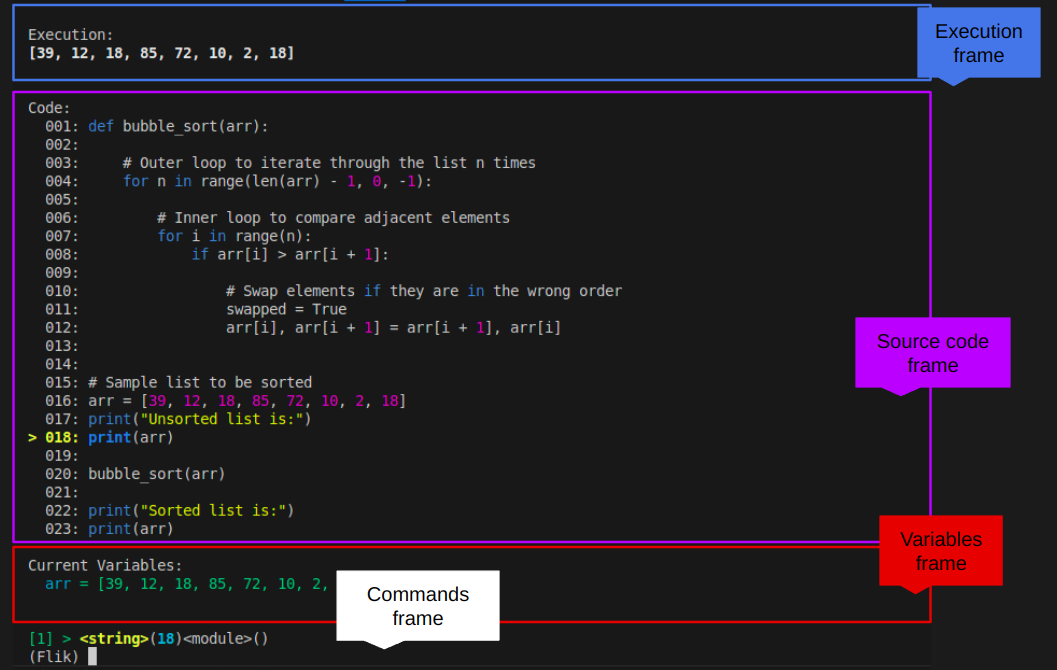
\includegraphics[width=1\textwidth]{figures/flik_interface.png}
    \caption{Debugger tool}
    \label{fig:debugger}
\end{figure}

% Add example of use step by step. Explain the videos.
% Now, let's use an example to further understand how \ac{Flik} works 


\endinput

